%!TEX root =../mapp-challenge-18-game-book.tex
% ^ leave for LaTeXTools build functionality

\phChapterWorksheet{Go Get 'Em!}{Main Puzzle 3}

While catching \mappMobimon{} on Interstate \(\sqrt{1.73205...}\),
you run across a wise old
\mappMobimon{} trainer who challenges you to a \mappMobimon{} battle. But not
just any \mappMobimon{} battle! This is a \textbf{puzzle battle.} The reward?
The location where all the \mappMobimon{} gather.

The old man tells you about a game he enjoyed in his youth called \textbf{Go.}

Go is a game of strategy played with black and white pieces on a grid. It's a
bit like chess, except instead of lots of kinds of pieces, each player only has
\textbf{one kind of piece, the stone.} And instead of playing on the squares,
players play on the \textbf{intersections of the grid lines,} and you can play
on board going from 9 by 9 up to 19 by 19. And \textbf{black goes first.} Maybe
it's not all that much like chess.

Much like chess, though, part of the strategy relies on \textbf{capturing your
  opponent's stones.} To capture you have to know about stones, groups of
stones, and their \textbf{liberties.}

Stones typically don't stay isolated for very long from other stones of the same
color. Stones form a \textbf{group} if they are \textbf{directly next to each
  other on the grid,} but \textbf{not diagonally.}

These stones form a group.

\begin{center}
  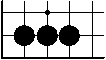
\includegraphics{gogetem/assets/explanation1-crop}
\end{center}

These stones \textbf{do not.} These are just three individual stones.

\begin{center}
  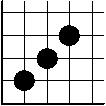
\includegraphics{gogetem/assets/explanation2-crop}
\end{center}

An individual stone has \textbf{liberties.} Liberties are the \textbf{empty
  spaces directly next to the stone on the grid,} but \textbf{not diagonally.}
So a stone may have \textbf{as many as 4} liberties. If an individual stone has
no liberties, \textbf{it is captured.}

The liberties of the black stones are marked with x's:

\begin{center}
  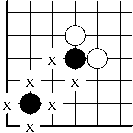
\includegraphics{gogetem/assets/explanation3-crop}
\end{center}

So the black stone on the lower left has \textbf{4 liberties,} and the black
stone on the upper right \textbf{only has two liberties} because the other two
spaces around it are occupied by white stones.

\textbf{Groups of stones share liberties.} A whole group of stones can be
captured at the same time if the whole group has no liberties. The group of
black stones below has \textbf{7 liberties.}

\begin{center}
  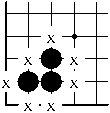
\includegraphics{gogetem/assets/explanation4-crop}
\end{center}

A stone can normally \textbf{not} be played in a space where it has no
liberties, with \textbf{one important exception.} A stone can be placed into a
space where it would have no liberties only if doing so \textbf{captures one or
  more enemy stones.}

The old man lays out several boards in an intermediate size, then says, ``In
each of the Go boards below, there is exactly one stone you can play, white or
black, that will allow you to make a capture. You need to figure out
\textbf{what color stone} to play and \textbf{where to play it} in order to make
a capture. Do that, and you will already know where all the \mappMobimon{}
gather.''

You notice that each of the boards the old man shows you is \textbf{13 by
  13.} There are also \textbf{26 letters in the alphabet.} Hmmm...

\begin{center}
  \contournumber{64}
  \begin{tikzpicture}
    \node[anchor=south west,inner sep=0] (image) at
    (0,0){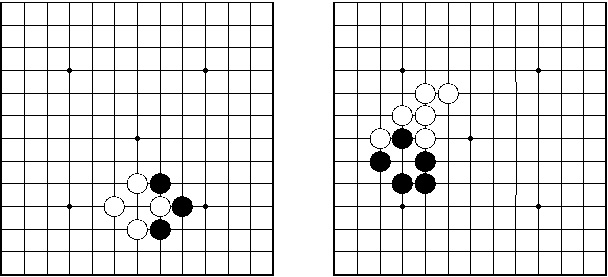
\includegraphics[scale=1.5]{gogetem/assets/boards1-crop}};
    % left board coordinate system
    \foreach \x in {0,...,12}
    \node at (\x * 0.58, 7.3){\contour{black}{\AlphAlph{\x + 14}}};
    \foreach \x in {0,...,12}
    \node at (-0.25, \x * 0.58){\contour{black}{\textcolor{white}{\AlphAlph{13 -
          \x}}}};
    % right board coordinate system
  \foreach \x in {0,...,12} \node at (8.5 + \x * 0.58,
  7.3){\contour{black}{\AlphAlph{\x + 14}}}; \foreach \x in {0,...,12} \node at
  (8.2, \x * 0.58){\contour{black}{\textcolor{white}{\AlphAlph{13 - \x}}}};
  \end{tikzpicture}

  \begin{tikzpicture}
    \node[anchor=south west,inner sep=0] (image) at
    (0,0){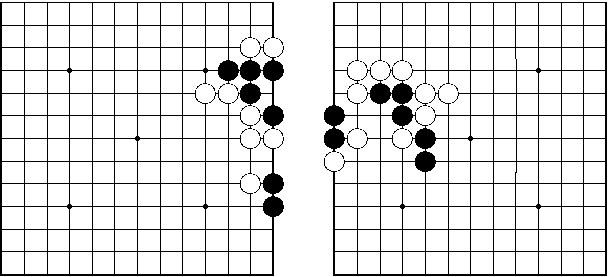
\includegraphics[scale=1.5]{gogetem/assets/boards2-crop}};
    % left board coordinate system
    \foreach \x in {0,...,12}
    \node at (\x * 0.58, 7.3){\contour{black}{\AlphAlph{\x + 14}}};
    \foreach \x in {0,...,12}
    \node at (-0.25, \x * 0.58){\contour{black}{\textcolor{white}{\AlphAlph{13 -
          \x}}}};
    % right board coordinate system
    \foreach \x in {0,...,12}
    \node at (8.5 + \x * 0.58, 7.3){\contour{black}{\AlphAlph{\x + 14}}};
    \foreach \x in {0,...,12}
    \node at (8, \x * 0.58){\contour{black}{\textcolor{white}{\AlphAlph{13 - \x}}}};
  \end{tikzpicture}

  \begin{tikzpicture}
    \node[anchor=south west,inner sep=0] (image) at
    (0,0){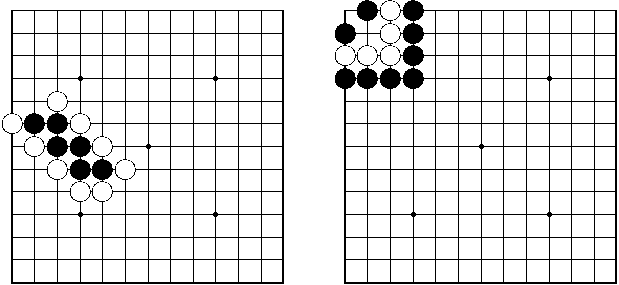
\includegraphics[scale=1.5]{gogetem/assets/boards3-crop}};
    % left board coordinate system
    \foreach \x in {0,...,12}
    \node at (\x * 0.58, 7.3){\contour{black}{\AlphAlph{\x + 14}}};
    \foreach \x in {0,...,12}
    \node at (-0.25, \x * 0.58){\contour{black}{\textcolor{white}{\AlphAlph{13 -
          \x}}}};
    % right board coordinate system
    \foreach \x in {0,...,12}
    \node at (8.7 + \x * 0.58, 7.5){\contour{black}{\AlphAlph{\x + 14}}};
    \foreach \x in {0,...,12}
    \node at (8.2, \x * 0.58){\contour{black}{\textcolor{white}{\AlphAlph{13 - \x}}}};
  \end{tikzpicture}

  \begin{tikzpicture}
    \node[anchor=south west,inner sep=0] (image) at
    (0,0){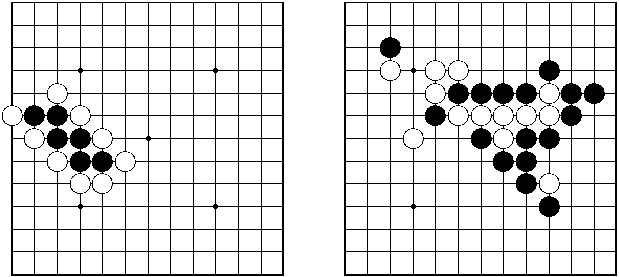
\includegraphics[scale=1.5]{gogetem/assets/boards4-crop}};
    % left board coordinate system
    \foreach \x in {0,...,12}
    \node at (0.3 + \x * 0.58, 7.5){\contour{black}{\AlphAlph{\x + 14}}};
    \foreach \x in {0,...,12}
    \node at (-0.25, \x * 0.58){\contour{black}{\textcolor{white}{\AlphAlph{13 -
          \x}}}};
    % right board coordinate system
    \foreach \x in {0,...,12}
    \node at (8.7 + \x * 0.58, 7.3){\contour{black}{\AlphAlph{\x + 14}}};
    \foreach \x in {0,...,12}
    \node at (8.2, \x * 0.58){\contour{black}{\textcolor{white}{\AlphAlph{13 - \x}}}};
  \end{tikzpicture}

  \begin{tikzpicture}
    \node[anchor=south west,inner sep=0] (image) at
    (0,0){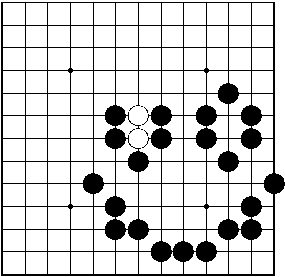
\includegraphics[scale=1.5]{gogetem/assets/boards5-crop}};
    % left board coordinate system
    \foreach \x in {0,...,12}
    \node at (\x * 0.58, 7.3){\contour{black}{\AlphAlph{\x + 14}}};
    \foreach \x in {0,...,12}
    \node at (-0.25, \x * 0.58){\contour{black}{\textcolor{white}{\AlphAlph{13 -
          \x}}}};
  \end{tikzpicture}

\end{center}
Where should you find the \mappMobimon{}?

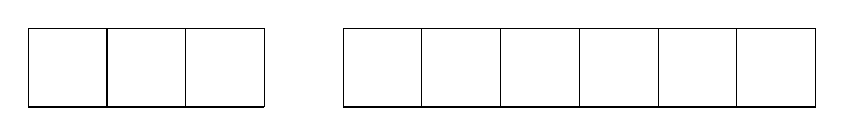
\begin{tikzpicture}
  \draw (0,0) grid (3,1);
  \draw (4,0) grid (10,1);
\end{tikzpicture}

% Include below for aucTeX integration
%%% Local Variables:
%%% mode: latex
%%% TeX-master: "../mapp-challenge-18-game-book"
%%% End:
